% SPDX-FileCopyrightText: 2026 Cyprien PIERRE
% SPDX-License-Identifier: CC-BY-4.0
\documentclass[tikz,border=5pt]{standalone}
\usepackage[T1]{fontenc}
\usepackage{lmodern}
\usetikzlibrary{arrows.meta,positioning}
\begin{document}
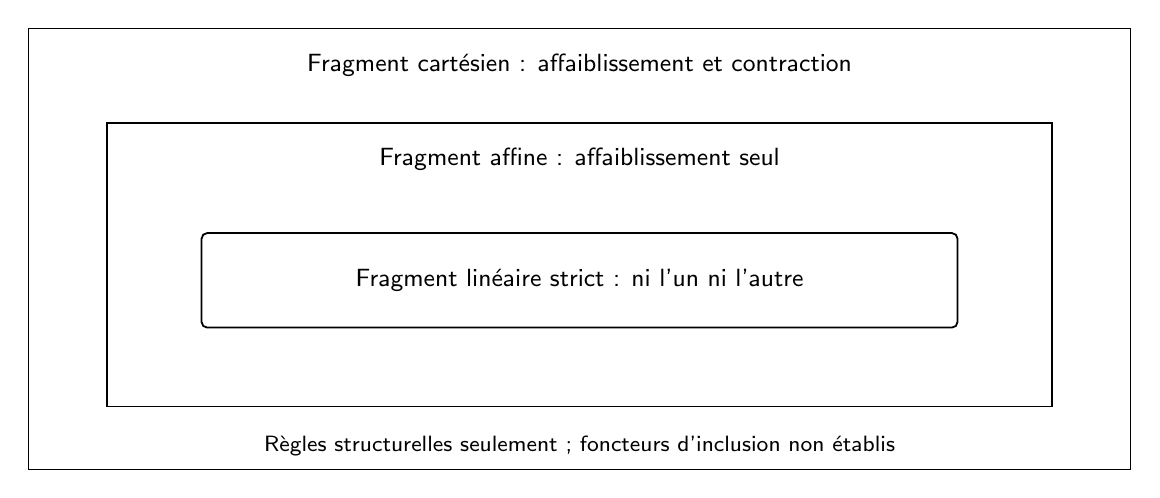
\begin{tikzpicture}[
  font=\sffamily\small,
  frame/.style={draw, line width=.5pt},
  box/.style={draw, rounded corners=2pt, align=center, line width=.65pt, minimum height=12mm}
]
\draw[frame] (0,0) rectangle (140mm,56mm);
\node[anchor=north] at (70mm,54mm) {Fragment cartésien : affaiblissement et contraction};
\draw[frame] (10mm,8mm) rectangle (130mm,44mm);
\node[anchor=north] at (70mm,42mm) {Fragment affine : affaiblissement seul};
\node[box, minimum width=96mm] at (70mm,24mm) {Fragment linéaire strict : ni l'un ni l'autre};
\node[align=center, font=\sffamily\footnotesize] at (70mm,3mm) {Règles structurelles seulement ; foncteurs d'inclusion non établis};
\end{tikzpicture}
\end{document}
